% spine = 0.0025 * 60 = 0.15
% Minimum Cover Width: Bleed + Back Cover Trim Size + Spine Width + Front Cover Trim Size + Bleed =  0.125" + 5" + 0.15" + 5" + .125" = 10.4''
% Minimum Cover Height: Bleed + Book Height Trim Size + Bleed = 0.125" + 8" + .125" = 8.25"
\documentclass[makeidx, 12pt, oneside, onecolumn, openright, final, svgnames, dvipsnames, extrafontsizes]{memoir}


\usepackage[mathjax]{lwarp}

\usepackage{pifont, dingbat}


\newcommand*\circnode[1]{\tikz[baseline=(char.base)]{%
            \node[shape=circle,fill=Olive!20,draw,inner sep=1.0pt] (char) {#1};}}

%\usepackage{smartdiagram}
%\usesmartdiagramlibrary{additions}


\usepackage{wrapfig2}
\usepackage{kantlipsum}

\title{Ancient Science Publishers}
\setcounter{tocdepth}{2} % Include subsections in the \TOC.
\setcounter{secnumdepth}{2} % Number down to subsections.
\setcounter{FileDepth}{2}
\booltrue{CombineHigherDepths}
\HTMLPageTop{\LinkPrevious}
\HTMLPageBottom{\LinkNext}
%\HTMLPageBottom{\LinkHome}

%\HTMLTitle{Ancient Science Publishers}



\CSSFilename{lwarp_sagebrush.css}

\usepackage[makeindex]{imakeidx} % hyper link index
\usepackage[colorlinks=true, linkcolor=ruddybrown, linktoc=all]{hyperref}% hyper link ToC

\PassOptionsToPackage{cmyk}{xcolor}
\usepackage{comment, calligra}
%\usepackage[paperheight=8.25in,paperwidth=10.4in,margin=0in]{geometry}
%\usepackage{pdfpages}
\usepackage{tikz, comment}
\usepackage{calligra, url, comment, amsmath, amsthm, etoolbox, amssymb, manfnt}
\usepackage{varwidth} % hyphenate texts in TikZ Node (back cover)
\usetikzlibrary{fadings, shadings, shadows, decorations, decorations.footprints, decorations.text, calc, positioning, mindmap,arrows, patterns, arrows.meta}
\usepackage{libertine}
\usepackage{fontspec}
%\usepackage[weather, misc]{ifsym}
%\usepackage{marvosym}
\usepackage{multido}
\usepackage{hologo, mflogo}
\usepackage[outline]{contour}
\usepackage{pdfrender}
\usepackage{pst-text}
\usepackage{pst-light3d}
\usepackage{pgfplots}
\pgfplotsset{width=5cm}
\usepackage{tikz-3dplot}
\usepackage{tkz-euclide}
\usepackage{tfrupee}
\usepgfplotslibrary{fillbetween}
\usepgfplotslibrary{polar}

%\usepackage{algorithm}
\usepackage{listings}


\setmainfont{Avant Garde}
\fontsize{0.05cm}{0.1cm}\selectfont

\usetikzlibrary{
  arrows,
  calc,
  fit,
  patterns,
  plotmarks,
  shapes.geometric,
  shapes.misc,
  shapes.symbols,
  shapes.arrows,
  shapes.callouts,
  shapes.multipart,
  shapes.gates.logic.US,
  shapes.gates.logic.IEC,
  circuits.logic.US,
  circuits.logic.IEC,
  circuits.logic.CDH,
  circuits.ee.IEC,
  datavisualization,
  datavisualization.formats.functions,
  er,
  automata,
  backgrounds,
  chains,
  topaths,
  trees,
  petri,
  mindmap,
  matrix,
  calendar,
  folding,
  fadings,
  shadings,
  spy,
  through,
  turtle,
  positioning,
  scopes,
  decorations.fractals,
  decorations.shapes,
  decorations.text,
  decorations.pathmorphing,
  decorations.pathreplacing,
  decorations.footprints,
  decorations.markings,
  shadows,
  shadows.blur,
  lindenmayersystems,
  intersections,
  fixedpointarithmetic,
  fpu,
  svg.path,
  external,
}


\newcommand*{\RaisedText}[1]{%
  \begingroup
    \leavevmode
    \rlap{\kern-1pt\raise.5pt\hbox{\color{White}#1}}%
    \rlap{\kern1pt\raise-.5pt\hbox{\color{black}#1}}%
    \hbox{#1}%
  \endgroup
}

\newcommand*{\RaisedTextNew}[1]{%
  \begingroup
    \leavevmode
    \rlap{\kern-.1pt\raise.1pt\hbox{%
      \pdfrender{
        TextRenderingMode=Stroke,
        LineWidth=.2pt,
        StrokeColor=white,
      }#1%
    }}%
    \rlap{\kern.1pt\raise-.1pt\hbox{%
      \pdfrender{
        TextRenderingMode=Stroke,
        LineWidth=.2pt,
        StrokeColor=black,
      }#1%
    }}%
    \rlap{%
      \pdfrender{
        TextRenderingMode=Stroke,
        LineWidth=.2pt,
      }#1%
    }%
    \hbox{#1}%
  \endgroup
}

\newfontfamily\hindifont[Script=Devanagari, BoldFont={Sahadeva}]{Nakula}
\newenvironment{hindi}{\hindifont}{\par}
\DeclareTextFontCommand{\texthindi}{\hindifont}

\tikzset{
  ld/.style={level distance=#1},lw/.style={line width=#1},
  level 1/.style={ld=4.5mm, trunk, lw=1ex ,sibling angle=60},
  level 2/.style={ld=3.5mm, trunk!80!leaf a,lw=.8ex,sibling angle=56},
  level 3/.style={ld=2.75mm,trunk!60!leaf a,lw=.6ex,sibling angle=52},
  level 4/.style={ld=2mm, trunk!40!leaf a,lw=.4ex,sibling angle=48},
  level 5/.style={ld=1mm, trunk!20!leaf a,lw=.3ex,sibling angle=44},
  level 6/.style={ld=1.75mm,leaf a, lw=.2ex,sibling angle=40},
}
\pgfarrowsdeclare{leaf}{leaf}{
  \pgfarrowsleftextend{-2pt} \pgfarrowsrightextend{1pt}
}{
  \pgfpathmoveto{\pgfpoint{-2pt}{0pt}}
  \pgfpatharc{150}{30}{1.8pt}
  \pgfpatharc{-30}{-150}{1.8pt}
  \pgfusepathqfill
}

\makeatletter
\def\agobble#1\nil#2{}
\def\mytextcolor@a#1 #2\nil#3{%
  \mytextcolor@b#1\nil{#3}
  \if\relax\detokenize{#2}\relax\expandafter\agobble\fi
  \mytextcolor@a#2\nil{#3}%
}
\def\mytextcolor@b#1#2\nil#3{%
  \textcolor{-#3}{\textbf{#1}}\textcolor{#3}{#2}\\
}
\def\mytextcolor#1#2{%
  \if\relax\detokenize{#2}\relax\expandafter\agobble\fi
  \mytextcolor@a#2 \nil{#1}%
}

\newcommand{\logo}[8]{%
  \colorlet{border}{#1}
  \colorlet{trunk}{#2}
  \colorlet{leaf a}{#3}
  \colorlet{leaf b}{#4}
%  \rotatebox{#8}{%
%    \begin{tikzpicture}[font=\scriptsize\scshape]
      \begin{scope}[scale=0.5, shift={(#8)}]
      \coordinate (root) [grow cyclic,rotate=90]
        child {
          child [line cap=round] foreach \a in {0,1} {
            child foreach \b in {0,1} {
              child foreach \c in {0,1} {
                child foreach \d in {0,1} {
                child foreach \leafcolor in {leaf a,leaf b}
                  { edge from parent [color=\leafcolor,-#5] }
                }
              }
            }
          }
          edge from parent [shorten >=-1pt,serif cm-,line cap=butt]
        };
      \node [scale=1,align=center,below,transform shape] at (0pt,-.5ex){%
        \mytextcolor{#6}{#7}\\
      };
    \end{scope}
%    \end{tikzpicture}
%  }
}
\makeatother


\tikzset{
    shade border west to east/.style args={#1 to #2}{
        preaction={draw, very thick, path fading=east, #1},
        preaction={draw, very thick, path fading=west, #2}
    },
    shade fill west to east/.style args={#1 to #2}{
        left color=#1,
        right color=#2
    }
}

\def\nodeshadowed[#1]#2;{\node[scale=0.45,above,#1]{#2};\node[scale=0.45,
        above,#1,yscale=-1,scope fading=south,opacity=0.0,yslant=0.0]{#2};}
        


%\definecolor{celestialblue}{rgb}{0.29, 0.59, 0.82}
\definecolor{celestialblue}{cmyk}{0.649, 0.274, 0.0, 0.164}

\definecolor{vividviolet}{rgb}{0.62, 0.0, 1.0}
\definecolor{satinsheengold}{rgb}{0.8, 0.63, 0.21}
\definecolor{darkorchid}{rgb}{0.6, 0.2, 0.8}
\definecolor{modebeige}{rgb}{0.59, 0.44, 0.09}

\newcommand{\hl}[1]{\textcolor{vividviolet}{#1}}% prints text in burntorange
\newcommand{\hlt}[1]{\textcolor{vividviolet}{\emph{#1}}}% prints italicized text in burntorange
\newcommand{\hlm}[1]{{\textcolor{modebeige}{#1}}}% prints math in Sepia
\newcommand{\hlbt}[1]{\textbf{\textcolor{Olive}{#1}}}% prints bold text in burntorange
%\newcommand{\hlmb}[1]{{\color{modebeige}{#1}}}% prints math in Sepia


% Inserts a blank page
\newcommand{\blankpage}{\newpage\hbox{}\thispagestyle{empty}\newpage}

\usepackage[mathcal]{euscript}
\newcommand{\conceptequiv}{\triangleq}
\CustomizeMathJax{\newcommand{\conceptequiv}{\triangleq}}
%\newcommand{\concepte}{\triangleq}
%\renewcommand{\models}{\looparrowright}
\renewcommand{\models}{\vDash}
\newcommand{\CC}{\mathcal{C}}
\CustomizeMathJax{\newcommand{\CC}{\mathcal{C}}}
\newcommand{\refines}{\looparrowright}
\CustomizeMathJax{\newcommand{\refines}{\looparrowright}}
\newcommand{\weakens}{\looparrowleft}
\CustomizeMathJax{\newcommand{\weakens}{\looparrowleft}}
\newcommand{\concept}[1]{\textcolor{Green}{#1}}

\newcommand\textproblem[1]{{\begin{center}\small \bfseries #1\end{center}}}


% no space ccenter
\newenvironment{nscenter}
 {\parskip=0pt\par\nopagebreak\centering}
 {\par\noindent\ignorespacesafterend}
 

\colorlet{LineColor}{White} 
\colorlet{FillColor}{Olive}%{DarkCyan}
%\colorlet{MyColor}{DarkOrange} 
%\colorlet{MyColor}{YellowOrange} 
\colorlet{MyColor}{Black}

\colorlet{TitleColor}{BurntOrange}
\colorlet{SubTitleColor}{Sepia}
\colorlet{DrawingTextColor}{Sepia}

\colorlet{AuthorTextColor}{Sepia}
\colorlet{BackTextColor}{Gray}
\colorlet{SpineTextColor}{Gray}

\colorlet{TriangleColor}{BurntOrange}
\colorlet{TriangleLineColor}{Sepia}
\colorlet{TriangleVertexColor}{Sepia}

\newcommand{\itemcolor}[1]{% Update list item colour
  \renewcommand{\makelabel}[1]{\color{#1}\hfil ##1}}
  
\newcommand\shadetext[2][]{%
  \setbox0=\hbox{{\special{pdf:literal 7 Tr }#2}}%
  \tikz[baseline=0]\path [#1] \pgfextra{\rlap{\copy0}} (0,-\dp0) rectangle (\wd0,\ht0);%
}

\newcommand{\aum}{\texthindi{ॐ}}
\newcommand{\Repeat}{\multido{\i=1+1}}

%\tikzfading[name=fade out,inner color=transparent!0,outer color=transparent!100]



\colorlet{EagleBodyColor}{White}
\colorlet{EagleHeadColor}{BurntOrange}
\colorlet{EagleEyeColor}{White}

\makeatletter
\tikzset{nomorepostaction/.code={\let\tikz@postactions\pgfutil@empty}}
\makeatother

\usepackage[capitalize,nameinlink]{cleveref}

\crefformat{chapter}{#2Dialogue~#1#3} % change cref to print Dialogue instead of Chapter

\newcommand\pr[1]{{\scshape\color{Black}\cref{#1}{ }(\cpageref{#1})}}
\newcommand\ar[1]{{\scshape\color{Black}\cref{#1}{ }(\cpageref{#1})}}
\newcommand\chref[1]{{\scshape\color{Black}\cref{#1}{ }(\cpageref{#1})}}

\newcommand\thmref[1]{{[\emph{\cref{#1}{ }(\cpageref{#1})}]}}
\newcommand\corref[1]{{[\emph{\cref{#1}{ }(\cpageref{#1})}]}}
\newcommand\exref[1]{{[\emph{\cref{#1}{ }(\cpageref{#1})}]}}

\definecolor{nicered}{rgb}{.647,.129,.149}
\definecolor{sanddune}{rgb}{0.59, 0.44, 0.09}
\definecolor{russet}{rgb}{0.5, 0.27, 0.11}
\makeatletter
\newlength\dlf@normtxtw
%\newcommand{\chapname}{Dialogue}
\setlength\dlf@normtxtw{\textwidth}
\def\myhelvetfont{\def\sfdefault{mdput}}
\newsavebox{\feline@chapter}
\newcommand\feline@chapter@marker[1][4cm]{%
  \sbox\feline@chapter{%
    \resizebox{!}{#1}{\fboxsep=1pt%
      \colorbox{sanddune}{\color{white}\bfseries\sffamily\thechapter}%
    }}%
  \rotatebox{90}{%
    \resizebox{%
      \heightof{\usebox{\feline@chapter}}+\depthof{\usebox{\feline@chapter}}}%
    {!}{\scshape\@chapapp}}\quad%
  \raisebox{\depthof{\usebox{\feline@chapter}}}{\usebox{\feline@chapter}}% 
}
\newcommand\feline@chm[1][4cm]{%
  \sbox\feline@chapter{\feline@chapter@marker[#1]}%
  \makebox[0pt][l]{% aka \rlap
    \makebox[0.0cm][r]{\usebox\feline@chapter}%
  }}
\makechapterstyle{daleif1}{
  \renewcommand\chapnamefont{\normalfont\Large\scshape\raggedleft\so}
  \renewcommand\chaptitlefont{\normalfont\huge\bfseries\scshape\color{Purple}}
  \renewcommand\chapternamenum{}
  \renewcommand{\chaptername}{Dialogue}
  %\renewcommand\printchaptername{\bfseries\color{DarkOrchid}}
  \renewcommand\printchaptername{\bfseries\color{russet}}
  \renewcommand\printchapternum{\null\hfill\feline@chm[2.5cm]\par}
  \renewcommand\afterchapternum{\par\vskip\midchapskip}
  \renewcommand\printchaptertitle[1]{\chaptitlefont\raggedleft ##1\par}
}
\makeatother

\setsecheadstyle{\normalfont\Large\bfseries\scshape\color{DarkOrchid}}


\chapterstyle{daleif1}
%\pagestyle{empty}

% Multi-page equations : mathmode by amsmath
\allowdisplaybreaks

\newenvironment{rcases}
  {\left.\begin{aligned}}
  {\end{aligned}\right\rbrace}
  
 \definecolor{ruddybrown}{rgb}{0.73, 0.4, 0.16} 
 
 \definecolor{xanadu}{rgb}{0.45, 0.53, 0.47}

\newtheoremstyle{problemstyle}  % <name>
        {0.2\baselineskip}                                               % <space above>
        {0.3\baselineskip}                                               % <space below>
        {\color{xanadu}}                               % <body font>
        {}                                                  % <indent amount}
        {\bfseries\color{xanadu}}                 % <theorem head font>
        {.}         % <punctuation after theorem head>
        {.5em}                                          % <space after theorem head>
        {}                                                  % <theorem head spec (can be left empty, meaning `normal')>
\theoremstyle{problemstyle}

  
  
\newtheorem*{pro}{\textbf{\S {} Problem}}%[chapter] 

\newenvironment{p}    % this is the environment name for the input
  {\renewcommand{\qedsymbol}{$\lozenge$}%
   \pushQED{\qed}\begin{pro}}
  {\popQED\end{pro}}
  
\definecolor{zinnwalditebrown}{rgb}{0.17, 0.09, 0.03}

\newenvironment{s}
  {\renewcommand{\qedsymbol}{\tiny$\blacksquare$}
  \vspace{-\baselineskip}\setmainfont{DejaVu Serif}\selectfont\begin{proof}[\emph{\textbf{\scshape\color{Black} \S \S \; Solution}}]}
  {\end{proof}} 
  
  

\DeclareMathOperator*{\Max}{Max}
\CustomizeMathJax{\DeclareMathOperator*{\Max}{Max}}
\DeclareMathOperator*{\Min}{Min}
\CustomizeMathJax{\DeclareMathOperator*{\Min}{Min}}

\usepackage{mleftright}
\usepackage[italicdiff]{physics} %careful: \div does not produce division symbol, it produces differential operator. Use \divisionsymbol for producing the division symbol.
  

\usepackage{algpseudocode}
\newcommand{\bigO}{\mathcal{O}}
\CustomizeMathJax{\newcommand{\bigO}{\mathcal{O}}}

\usepackage{enumitem}

\definecolor{applegreen}{rgb}{0.55, 0.71, 0.0}
%\definecolor{armygreen}{rgb}{0.29, 0.33, 0.13}
\definecolor{auburn}{rgb}{0.43, 0.21, 0.1}

\newenvironment{defn}
  {\renewcommand{\qedsymbol}{{\color{auburn}\tiny$\blacksquare$}}\vspace{-0.4\baselineskip}\begin{proof}[\emph{\textbf{\scshape\color{auburn} \underline{Definition}}}]\color{applegreen}}
  {\end{proof}}
  
\usepackage{epigraph}





\makeatletter
\begin{document}
\pagestyle{empty}

\setmainfont{DejaVu Serif}
%\fontsize{0.5cm}{0cm}\selectfont

\pgfkeyssetvalue{/cfr/soul base dimension}{10pt}

\begin{center}
\begin{tikzpicture}[remember picture,overlay]


%\begin{scope}[scale=1.9, xshift=3.95in,yshift=-1.75in,color=TriangleLineColor]
%\begin{scope}[xshift=3.95in, color=TriangleLineColor]
\begin{scope}[scale=1, shift={(current page.center)}]

   
     \begin{scope}[scale=3.5, rotate=180, yshift=-0.77in]
        \tkzDefPoint(0,1){J} \tkzDefPoint(0,0){O}
        \foreach \i in {0,-1,-2,...,-180}{
        \tkzDefPoint({2.1*cos(\i*3.14159/180)},{1+2.1*sin(\i*3.14159/180)}){P}
        \tkzDrawLine[color=TriangleColor, thick](J,P)}
    \end{scope}

     \begin{scope}[scale=1, yshift=4.8in]
 \newcounter{density}
 \setcounter{density}{90}
\tkzDefPoint(0,0){G1}
    \tkzDefPoint(-120:5){G2}
    \tkzDefPoint(-60:5){G3}   
    
        \tkzLabelPoint[above,color=TriangleVertexColor](G1){\color{Red} \bfseries \HUGE \texthindi{ॐ}}
    \tkzLabelPoint[left,color=TriangleVertexColor](G2){\color{Red} \HUGE \texthindi{ॐ}}
    \tkzLabelPoint[right,color=TriangleVertexColor](G3){\color{Red} \HUGE \texthindi{ॐ}}
    
    \tkzDrawPoints[color=TriangleColor](G1,G2,G3)
    
    \tkzDrawPolygon(G1,G2,G3)      
        
    \path[coordinate, fill=TriangleColor, draw=TriangleLineColor] (0,0)   coordinate(G1)
                -- (-120:5) coordinate(G2)
                -- (-60:5) coordinate(G3);
    
    \tkzLabelSegment[above,sloped,midway](G2,G1) {\calligra \LARGE  \color{Sepia} \texthindi{प्राचीन}}
    \tkzLabelSegment[above,sloped,midway](G1,G3) {\calligra \LARGE \color{Sepia}  \texthindi{विज्ञान}}
    \tkzLabelSegment[below,sloped,midway](G2,G3) {\calligra \LARGE \color{Sepia}  \texthindi{मण्डल}}
    
    \foreach \x in {1,...,10}
    {%
    \pgfmathsetcounter{density}{\thedensity-10}
    \setcounter{density}{\thedensity}
    \path[coordinate, color=TriangleColor] coordinate(X) at (G1){};
    \path[coordinate, ball color=TriangleColor, draw=TriangleLineColor] (G1) -- (G2) coordinate[pos=.15](G1)
                        -- (G3) coordinate[pos=.15](G2)
                        -- (X) coordinate[pos=.15](G3);
    \draw[->,ball color=TriangleColor, draw=TriangleLineColor, fill=TriangleColor!\thedensity]  (G1)--(G2)--(G3)--cycle;
    }     
     
\node[scale=2.1, at={(0in, -2.5in)}]
    {\bfseries \textcolor{TriangleColor}{\RaisedText{Ancient Science Publishers}}};
    
\node[scale=1.9, at={(0in, -3.2in)}]
    {\bfseries \textcolor{Sepia}{\calligra {Decode The Myth}}};

%\node[text=Yellow,scale=0.9] at(0in, -4.2) {
%\begin{varwidth}{6cm}
% \Letter \, \texttt{ancientsciencepublishers@gmail.com}\\
%\Telefon \, \texttt{+91 9353015055}
%\end{varwidth}

\node[scale=1.0, at={(0in, -4.8in)}]
{\HUGE \bfseries \color{TriangleColor}{\RaisedText{\texthindi{अन्तर्चक्षुः}}}};

\node[scale=0.8, at={(0in, -5.4in)}]
{\HUGE  \color{TriangleColor}{\RaisedText{\texthindi{भगवान् महर्षि हिरण्यगर्भ}}}};

\node[scale=1.0, at={(0in, -6.2in)}]
{\HUGE \bfseries \color{TriangleColor}{\RaisedText{Beacons of Light}}};

\node[scale=0.8, at={(0in, -6.8in)}]
{\HUGE \bfseries \textcolor{TriangleColor}{\calligra\RaisedText{Edsger Wybe Dijkstra}}};

\node[scale=0.8, at={(0in, -7.4in)}]
{\HUGE \bfseries \textcolor{TriangleColor}{\calligra\RaisedText{Richard Phillips Feynman}}};

\node[scale=0.8, at={(0in, -8in)}]
{\HUGE \bfseries \textcolor{TriangleColor}{\calligra\RaisedText{Leonhard Euler}}};


\node[scale=1.0, at={(0in, -9.4in)}]
{\HUGE \bfseries \color{TriangleColor}{\RaisedText{Artifacts}}};

\node[scale=0.8, at={(0in, -10in)}]
{\HUGE \bfseries \textcolor{TriangleColor}{\calligra\RaisedText{Monographs}}};
\end{scope} 
\end{scope}


%\node[scale=1.0, at={(0in, -1.3in)}]
%{\HUGE \bfseries \textcolor{TriangleColor}{\calligra\RaisedText{Richard Phillips Feynman}}};

%\node[scale=1.0, at={(0in, -3.1in)}]
%{\HUGE \bfseries \textcolor{TriangleColor}{\calligra\RaisedText{Leonhard Euler}}};

\end{tikzpicture}
\end{center}

\frontmatter

\begin{center}
\Large \href{mailto:ancientsciencepublishers@gmail.com}{\nolinkurl{ancientsciencepublishers@gmail.com}}
\end{center}

%\begin{wrapfigure}{r}{0.5\textwidth}
  \begin{center}
    
\includegraphics[width=1.0\textwidth]{catalogue/asp-catalogue}
  \end{center}
  %\caption{Front Cover}
%\end{wrapfigure}


\renewcommand{\contentsname}{Monographs}

\pagenumbering{gobble}
\tableofcontents*


\mainmatter

\setlength{\headwidth}{\textwidth}
\setlength{\headwidth}{\textwidth}

\renewcommand{\chaptername}{Monograph}

\part{\textcolor{red}{Computer Science}}

\chapter{Discipline of Competitive Programming : A Hacker’s Perspective}
%\begin{wrapfigure}{r}{0.5\textwidth}
  \begin{center}
    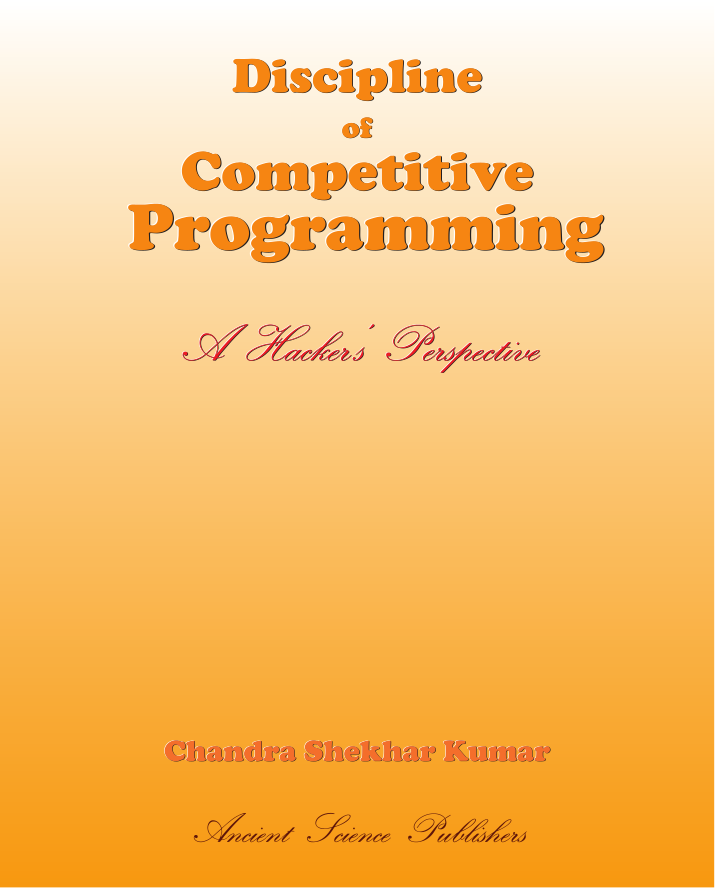
\includegraphics[width=0.8\textwidth]{dcp/cover}
  \end{center}
  %\caption{Front Cover}
%\end{wrapfigure}


\chapter{Elements of Coding : Science of Deriving Correct Programs}
%\begin{wrapfigure}{r}{0.5\textwidth}
  \begin{center}
    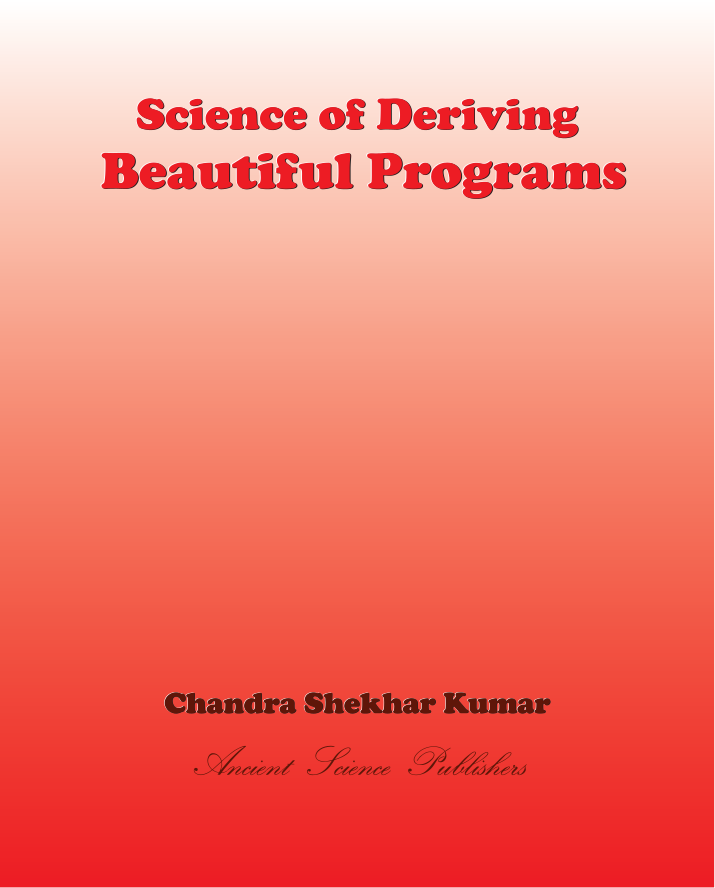
\includegraphics[width=0.8\textwidth]{science-dcp/cover}
  \end{center}
  %\caption{Front Cover}
%\end{wrapfigure}


\chapter{Elements of Coding Linear Algebra : The Nucleus of Artificial Intelligence}
%\chapter{Algebraic Concepts}
%\label{ch1}
%\thispagestyle{empty}
%\protected@edef\concepteq{%
%\[\conceptequiv\]
%}

\underline{\textcolor{BurntOrange}{\textbf{Excerpt from the Chapter \Large \textcolor{Sepia}{Algebraic Concepts}}}}

\vspace{5mm}

\hspace{4mm}\hlt{\textbf{Concept} $\mathcal{C}$ is a predicate describing a set of syntactic and semantic requirements on related types ($<T_i>$) together with a collection of similar procedures $\left(f : T^i \rightarrow T^j\right)$ stated in terms of the properties, attributes and type functions $\left(F : \mathcal{C}^i \rightarrow \mathcal{C}^j \right)$ defined on the types.}
\begin{gather*}
\therefore \mathcal{C}\left(<T_i>\right) \conceptequiv \wedge <\Psi_j>
\end{gather*}
where $\conceptequiv$ stands for \hlt{is defined by} and the $\Psi_j$ represent independent clauses defining the concept.

\begin{lstlisting}
template<class T>
    concept integral = is_integral_v<T>;
\end{lstlisting}

\hlt{If a type $T$ fulfills all the requirements of a concept $\mathcal{C}$, then $T$ \textbf{models} $\mathcal{C}$}, i.e. $T \models \CC$.

\begin{nscenter}
int8\_t and uint8\_t $\models$ \concept{integral}.
\end{nscenter}

\hlt{Concept $\mathcal{C}^i$ is a \textbf{refinement} of concept $\mathcal{C}^j$ if it subsumes the latter, i.e. if $\mathcal{C}^i$ is true for a set of types, then $\mathcal{C}^j$ is also true for the same set.}

In other words, $\mathcal{C}^i$ \hlt{refines} $\mathcal{C}^j$ ($\mathcal{C}^i \refines \mathcal{C}^j$) by addition of more requirements to $\mathcal{C}^j$, i.e. $\mathcal{C}^j$ \hlt{weakens} $\mathcal{C}^i$ ($\mathcal{C}^j \weakens \mathcal{C}^i$). 

\begin{lstlisting}
template<class T>
    concept signed_integral = integral<T> && is_signed_v<T>;
\end{lstlisting}

\begin{nscenter}
\concept{signed\_integral} $\refines$ \concept{integral} \\
int8\_t $\models$ \concept{signed\_integral}  
\end{nscenter}

\begin{lstlisting}
template<class T>
concept unsigned_integral = integral<T> && !signed_integral<T>;
\end{lstlisting}

\begin{nscenter}
\concept{unsigned\_integral} $\refines$ \concept{integral} \\
uint8\_t $\models$ \concept{unsigned\_integral}  
\end{nscenter}




\begin{comment}

{\color{plotptcolor}
\vspace{1in}

\hrule
\vspace{1mm}
\hrule

\fancybreak{$\blacktriangle\blacktriangle\blacktriangle$}
\begin{hindi}
\centering \bfseries\large 
ॐ 
\end{hindi}
\fancybreak{$\blacktriangledown\blacktriangledown\blacktriangledown$}

\hrule
\vspace{1mm}
\hrule}
\end{comment}






\chapter{Elements of Software Design Patterns}
%\begin{center}
\begin{wrapfigure}{r}{0.5\textwidth}
\begin{tikzpicture}[remember picture,overlay]
\begin{scope}[shift={(current page.center)}]
  \node[scale=.6, at={(2.8in, 3.4in)}]
    {\setmainfont{Cooper Black}
\fontsize{2cm}{1.5cm}\selectfont \bfseries {\textcolor{Snow}{\RaisedText{\calligra{Elements}}}}};

\node[scale=.6, at={(2.8in, 2.7in)}]
    {\setmainfont{Cooper Black}
\fontsize{2cm}{1.5cm}\selectfont \bfseries {\textcolor{Snow}{\RaisedText{\calligra{of}}}}};

\node[scale=0.65, at={(3.0in, 2.1in)}]
    {\setmainfont{Cooper Black}
\fontsize{2cm}{1.5cm}\selectfont \bfseries \textcolor{Snow}{\RaisedText{Software Design}}};

\node[scale=0.9, at={(3.0in, 1.3in)}]
    {\setmainfont{Cooper Black}
\fontsize{2cm}{1.5cm}\selectfont \bfseries \textcolor{Snow}{\RaisedText{Patterns}}};


\node[scale=0.4, at={(3in, -2.7in)}]
    {\setmainfont{Cooper Black}
\fontsize{2cm}{1.5cm}\selectfont \bfseries \textcolor{Snow}{\RaisedText{Chandra Shekhar Kumar}}};


\node[scale=0.3, at={(3in, -3.1in)}]
    {\setmainfont{Cooper Black}
\fontsize{2cm}{1.5cm}\selectfont \bfseries \textcolor{Black}{\calligra {Ancient Science Publishers}}};

%design spine 
\node[scale=0.8, rotate=-90,  minimum width=9.3in, minimum height=0.9in,ultra thick] 
at(0,-0.0) 
{
\setmainfont{Cooper Black}
\fontsize{1.0cm}{0.5cm}\selectfont
\begin{varwidth}{17in}
\color{Snow}
\RaisedText{Elements of Software Design Patterns}
\end{varwidth}
};

\begin{scope}[remember picture, xshift=5cm]
\node[ellipse callout, callout pointer shorten=-1.2cm, draw] (hallo) 
{
\begin{varwidth}{1.8in}
I am a pattern.

What are you?
\end{varwidth}
};

\draw[fill=Grey] (-0.5,-4.5) circle [x radius=1.5cm, y radius=5mm];
\draw[fill=Grey] (5,-4.5) circle [x radius=1cm, y radius=5mm];

\begin{scope}[xshift=-3.5cm, yshift=-0.5cm]
\begin{scope}[y=0.80pt, x=0.80pt, yscale=-0.5, xscale=0.5, inner sep=0pt, outer sep=0pt]
\path[draw, fill=Black,even odd rule] (386.4600,182.7600) .. controls (380.5260,182.3640) and (374.0910,184.0390) .. (369.4330,187.7910) .. controls (370.8200,185.4800) and (372.2190,183.4020) .. (373.3020,180.8250) .. controls (366.6320,180.9420) and (360.7610,183.0510) .. (354.6830,185.5840) .. controls (348.1310,188.3130) and (343.0510,182.0710) .. (337.6970,178.5020) .. controls (328.5990,172.4380) and (318.4820,166.3890) .. (313.4880,156.4000) .. controls (308.9610,147.3470) and (301.9760,127.8640) .. (288.2940,129.4720) .. controls (274.2360,131.1270) and (266.4640,123.6190) .. (255.6510,115.8070) .. controls (234.7890,100.7320) and (215.7280,82.8280) .. (188.6990,79.4280) .. controls (161.5340,76.0120) and (135.6750,88.4450) .. (111.4310,98.4280) .. controls (88.7860,107.7520) and (59.5580,119.9360) .. (38.5410,100.3270) .. controls (29.3610,91.7620) and (24.5120,78.5840) .. (21.3670,66.7900) .. controls (17.6240,52.7560) and (24.3950,44.3350) .. (29.9910,32.3460) .. controls (32.4580,27.0580) and (32.3670,-3.2680) .. (21.7070,0.2850) .. controls (12.1280,3.4770) and (12.2530,24.5660) .. (8.6270,32.5420) .. controls (2.6690,45.6470) and (-0.8060,55.1290) .. (0.1620,69.6300) .. controls (0.9820,81.9410) and (6.9130,94.8560) .. (12.9940,105.3670) .. controls (36.1080,145.3280) and (85.7680,142.4600) .. (124.8340,130.1370) .. controls (121.7750,141.9320) and (125.0470,150.5490) .. (127.3430,162.0300) .. controls (128.4310,167.4730) and (128.2430,173.0530) .. (129.0920,178.5120) .. controls (130.1360,185.2330) and (134.1230,190.1210) .. (135.6710,196.3150) .. controls (137.6700,204.3080) and (138.8680,219.8830) .. (134.3170,227.4690) .. controls (127.4420,238.9280) and (134.7940,243.6040) .. (136.0590,254.7530) .. controls (137.2200,264.9820) and (132.6560,275.9590) .. (146.5080,278.3600) .. controls (151.6900,279.2580) and (161.6800,278.2010) .. (164.3100,272.9420) .. controls (168.6440,264.2730) and (161.0060,267.7030) .. (157.5380,264.2340) .. controls (154.8410,261.5390) and (155.0530,252.9090) .. (153.7750,249.0760) .. controls (151.8480,243.2950) and (152.3330,237.9310) .. (154.4420,232.3060) .. controls (158.2770,222.0780) and (166.6630,211.8920) .. (165.0850,200.5710) .. controls (172.1600,211.9720) and (172.4630,221.7580) .. (166.6330,233.8540) .. controls (164.2230,238.8550) and (159.8630,243.8760) .. (161.6020,250.1080) .. controls (162.6430,253.8370) and (165.9040,254.9870) .. (167.7940,257.8480) .. controls (169.8990,261.0370) and (170.7110,264.4470) .. (172.9970,267.4940) .. controls (181.1970,278.4280) and (187.5520,285.7130) .. (202.2380,285.7130) .. controls (208.3370,285.7130) and (212.7340,285.6950) .. (214.2360,278.9410) .. controls (215.8780,271.5520) and (210.7010,270.5280) .. (204.6940,268.9260) .. controls (197.9420,267.1260) and (193.3560,267.9050) .. (190.6280,260.5570) .. controls (188.3880,254.5250) and (189.6850,247.1190) .. (190.5070,240.9530) .. controls (190.9980,237.2670) and (198.1880,229.5340) .. (200.3030,226.1140) .. controls (203.5980,220.7850) and (206.0530,215.3790) .. (209.0320,209.9170) .. controls (217.8900,193.6780) and (226.3260,216.5620) .. (229.9080,226.1140) .. controls (233.9870,236.9900) and (233.4210,253.3020) .. (240.9380,262.1060) .. controls (245.2300,267.1320) and (266.0050,272.2320) .. (265.3190,260.5570) .. controls (264.9940,255.0270) and (254.8840,254.8990) .. (252.5480,251.6560) .. controls (249.7520,247.7760) and (252.5480,239.9970) .. (252.5480,235.4020) .. controls (256.0660,240.3200) and (259.3810,245.7330) .. (263.9000,249.7510) .. controls (268.9880,254.2720) and (269.2890,259.9800) .. (272.6730,265.5890) .. controls (279.3290,276.6240) and (288.1900,281.6540) .. (300.7940,276.0530) .. controls (305.0600,274.1570) and (302.2120,266.1600) .. (299.1820,264.4280) .. controls (292.9670,260.8760) and (290.5570,266.5530) .. (287.3780,259.0100) .. controls (283.2070,249.1100) and (283.6690,235.3660) .. (282.1530,224.7590) .. controls (281.6320,221.1110) and (292.9140,225.4690) .. (296.0860,225.6670) .. controls (301.0350,225.9760) and (309.7770,223.9760) .. (314.0810,225.3410) .. controls (318.7460,226.8200) and (321.0190,233.0080) .. (324.5310,236.1760) .. controls (329.6070,240.7570) and (335.3810,244.3040) .. (342.3760,244.3040) .. controls (353.9930,244.3040) and (358.2910,259.8880) .. (372.5200,254.7530) .. controls (375.6520,253.6230) and (382.3360,250.9170) .. (382.7760,247.4000) .. controls (383.5000,241.6150) and (378.4720,237.9130) .. (379.8740,232.3060) .. controls (381.9430,224.0280) and (378.0000,215.0970) .. (375.6170,207.1510) .. controls (373.7900,201.0560) and (372.8770,198.9840) .. (377.3590,193.6040) .. controls (380.2590,190.1440) and (383.1690,185.8940) .. (386.4590,182.7940);




\path[draw=black,fill=Snow,even odd rule,line width=0.249pt,miter limit=5.33] (374.8400,224.5600) .. controls (370.1790,224.1080) and (362.2460,225.3020) .. (365.5520,231.9140) .. controls (369.9820,240.7540) and (373.5020,228.1540) .. (374.8420,224.5640);



\path[draw=black,line cap=rect,line width=0.249pt,miter limit=5.33] (382.5800,245.8400) .. controls (385.0340,240.3050) and (389.2710,235.2550) .. (394.5780,232.2960);



\path[draw=black,line cap=rect,line width=0.249pt,miter limit=5.33] (376.0000,248.9400) .. controls (365.0840,249.4720) and (356.6660,254.6200) .. (348.9100,262.0980);



\path[draw=black,line cap=rect,line width=0.249pt,miter limit=5.33] (367.8800,245.8400) .. controls (359.2980,247.8990) and (350.4040,248.1800) .. (341.9500,250.4850);



\path[draw=black,line cap=rect,line width=0.249pt,miter limit=5.33] (360.9100,250.1000) .. controls (352.0790,251.4510) and (343.5320,253.4170) .. (335.3680,257.0670);



\path[draw=black,fill=Black,even odd rule,line width=0.249pt,miter limit=5.33] (382.9700,244.3000) .. controls (379.9050,245.1640) and (379.0350,248.1570) .. (376.0040,248.9450) .. controls (378.8140,253.6450) and (383.9040,249.0350) .. (382.9740,244.3050);



\path[draw=black,fill=Black,even odd rule,line width=0.249pt,miter limit=5.33] (370.9700,224.9500) .. controls (371.4990,228.0060) and (370.8810,231.0770) .. (368.6490,233.0770) .. controls (369.1990,229.9370) and (368.8390,225.8270) .. (370.9690,224.9470);
\end{scope}
\end{scope}
\begin{scope}[xshift=5cm]
\node[ellipse callout, callout relative pointer={(0,-1)}, draw] (hallo) 
{
\begin{varwidth}{1.5in}
Quality \\without \\ a name!
%\texthindi{मैं बहुरुपिया कोरोना।}
\end{varwidth}
};
\end{scope}
\end{scope}
\end{scope}
\end{tikzpicture}
%\end{center}
\end{wrapfigure}

\underline{\textbf{\textcolor{BurntOrange}{Excerpt from the Chapter} \textcolor{Sepia}{(Pattern Concept):}}}

\begin{defn}
A pattern is a rule triad expressing a relation between:
\begin{enumerate}
  \item a certain \hlt{context} defining the scope of applicability of the given pattern,
  \item a \hlt{problem} detailing a certain system of conflicting forces which occurs repeatedly that the pattern resolves in that context and
  \item a \hlt{solution} in a form of a certain software configuration which can be used repeatedly and uniquely to resolve the given system of forces themselves, wherever the context makes it relevant.
\end{enumerate}
\par\vspace{-1.8\baselineskip}
\qedhere
\end{defn}

%\begin{warpHTML}
\begin{wrapfigure}{l}{0.5\textwidth}
  \begin{center}
    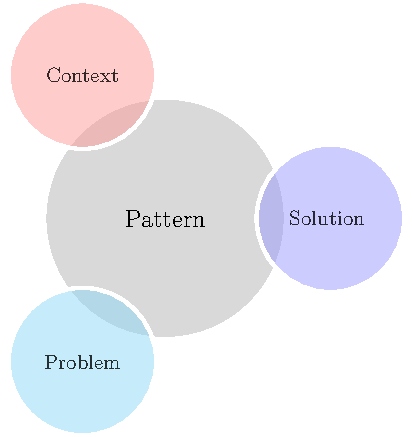
\includegraphics[width=0.5\textwidth]{designpatterns/patterns-triad}
  \end{center}
  %\caption{Front Cover}
\end{wrapfigure}
%\end{warpHTML}


The output of this rule triad is a pattern too.

\vspace{4mm}

It leads (but not limited) to the following  key observations about pattern:
%\begin{enumerate}[label=\protect\circnode{\color{red}\arabic*}]
\begin{dinglist}{213}
\item It is both a thing and a process.
\item It is both a description of a thing which is alive and a description of the process which will generate that thing.
\item It is both a thing which happens in the world and the rule which tells us how to create that thing.
\item It can exist at all scales and resolve almost any kind of conflicting forces.
\item Identification of what-why-when-where marks its inner structure explicit and sharable.
\item It starts with defining features worth abstracting.
\item Then it defines the problem, i.e. the field of forces which it brings into balance.
\item It is a sketch rather than a blue-print. 
\item It can complement and compound another pattern(s).
\item It is generative and self-sustaining.
\item It is a micro-architecture.
\item It promotes design-reuse.
\item The exact range of contexts is defined where the stated problem occurs and where this particular solution to the problem is appropriate.
\item Each pattern describes a problem which occurs over and over again in our system and then describes the core of the solution to that problem in such a way that we can use this solution a million times over, without ever doing it the same way twice.
\end{dinglist}

Beyond its elements, each system is defined by a certain patterns of relationships among the elements, and these relationships are integral part of the elements to such an extent that the elements themselves are patterns of relationships. And finally, the so called elements get dissolved, leaving patterns of relationships behind, which is the actual thing that actually repeats itself and gives structure to the system.

Each one of these patterns $\mathcal{P}_i$  is a morphological law onto itself, which establishes a set of relationships in the system in a given context of type $\mathcal{C}$, i.e.
\hlm{\begin{gather*}
\mathcal{P}_i \triangleq \mathcal{C} \rightarrow \mathcal{R}\left(\ldots, \mathcal{P}_{i-1}, \mathcal{P}_{i+1}, \ldots\right)
\end{gather*}} 
where $\triangleq$ stands for \hlt{is defined by}. The parts (i.e, rest of the patterns except $\mathcal{P}_i$) $\ldots, \mathcal{P}_{i-1}, \mathcal{P}_{i+1}, \ldots$ are related by the relationship $\mathcal{R}$ within a context of type $\mathcal{C}$.

Note that, each law or pattern is itself a pattern of relationships among the remaining laws (i.e. except itself), which are themselves just patterns of relationships again.

\hlt{Therefore, a pattern is defined by formulating it in the form of a rule triad as depicted before,  which establishes a relationship between a context, a system of (often conflicting) forces which arise in that context and configuration which allows these forces to resolve themselves in that context.}

\vspace{3mm}

Hence, generic form of each pattern is:

%\begin{wrapfigure}{r}{0.5\textwidth}
  \begin{center}
    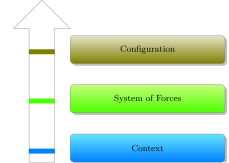
\includegraphics[width=0.7\textwidth]{designpatterns/patterns-form}
  \end{center}
  %\caption{Front Cover}
%\end{wrapfigure}

Discovery of (the invariant features) pattern(s) always start with observation or purely abstract argument. This process is not sequential from the problem to the solution or vice versa. Rather it is a multidimensional global process to help identify a solid and reliable invariant which relates context, problem, solution in an unchanging way. 

The statement of the problem and the forces helps to solidify the pattern which is responsible for making the system of forces come to an equilibrium. Thought it is still tentative, but clear enough to be shared.

There are two components in a pattern definition, which are empirical in nature, i.e. can be tested as true/false:
\begin{enumerate}
\item The problem is real, i.e. it is expressible as conflicting real forces within the stated context(s).
\item The configuration solves the problem, i.e. it deals with all the forces in the stated context(s).
\end{enumerate}
Quality without a name is the living essence of a pattern.

\vspace{20mm}

\underline{\textbf{\textcolor{BurntOrange}{Excerpt from the Chapter} \textcolor{Sepia}{(Pattern Form):}}}

\hspace{5mm}Each (living) pattern has the same form for the sake of convenience and clarity. It has \hlt{nine} parts in the following sequence :
\begin{enumerate}[label=\protect\circnode{\color{Sepia}\arabic*}]
\item A \hlt{picture} is drawn to illustrate an archetypal example of the pattern.
\item An \hlt{introductory paragraph} to set the context for the pattern.
\item The symbol \hl{\texthindi{ॐ}} marks the beginning of the problem the pattern addresses later.
\item A \hlbt{headline} set in bold-typeface to provide the essence of the problem.
\item The \hlt{body} of the problem describing (but not limited to) the 
    \begin{dinglist}{213}
        \item empirical background of the pattern,
        \item empirical evidence for its validity which sets the motivational tone too,
        \item variations, i.e. the range of different ways of manifesting it in a software.
    \end{dinglist}
\item The \hlbt{solution} set in bold-typeface, encoded in an instructional form, stating the exact steps to build the pattern. It illustrates the field of relationships needed to solve the stated problem in the stated context.
\item A \hlt{diagram} that shows the solution as a labeled picture indicating its main components.
\item The symbol \hl{\texthindi{ॐ}} marking the end of the main body of the pattern.
\item A \hlt{paragraph}, which ties the pattern to all those smaller patterns in the pattern language, which are needed to complete this pattern, to embellish it, to fill it out.
\end{enumerate}

This form serves the following two essential purposes :
\begin{enumerate}[itemsep=0.3em]%[label=\protect\circnode{\color{Sepia}\arabic*}]
    \item to present each pattern connected to other patterns to help grasp the collection of all these patterns as a whole, as a pattern language, within which an infinite variety of combinations can be created.
    \item to present the problem and solution of each pattern in such a way that it sets the exact tone of self-judgment and modifications without losing the central essence. 
\end{enumerate}

\vspace{20mm}

\underline{\textbf{\textcolor{BurntOrange}{Excerpt from the Chapter} \textcolor{Sepia}{(Null Object):}}}

\epigraphhead[30]
{
\epigraph{\hlt{Do what you can to establish coherence in your software. I am smart because I do nothing!}}{}

}

\begin{center}
\begin{tikzpicture}[remember picture]
\node[ellipse callout, callout pointer shorten=-1.2cm, draw] (hallo) 
{
\begin{varwidth}{1.5in}
I am a reference!

What are you?
%\begin{hindi}
%मैं वैक्सीन हूँ। 

%तू कौन है?
%\end{hindi}
\end{varwidth}
};

\draw[fill=Grey] (-0.5,-4) circle [x radius=1.5cm, y radius=5mm];
\draw[fill=Grey] (5,-4) circle [x radius=1cm, y radius=5mm];

\begin{scope}[xshift=-3.5cm]
\begin{scope}[y=0.80pt, x=0.80pt, yscale=-0.5, xscale=0.5, inner sep=0pt, outer sep=0pt]
\path[draw, fill=Orange,even odd rule] (386.4600,182.7600) .. controls (380.5260,182.3640) and (374.0910,184.0390) .. (369.4330,187.7910) .. controls (370.8200,185.4800) and (372.2190,183.4020) .. (373.3020,180.8250) .. controls (366.6320,180.9420) and (360.7610,183.0510) .. (354.6830,185.5840) .. controls (348.1310,188.3130) and (343.0510,182.0710) .. (337.6970,178.5020) .. controls (328.5990,172.4380) and (318.4820,166.3890) .. (313.4880,156.4000) .. controls (308.9610,147.3470) and (301.9760,127.8640) .. (288.2940,129.4720) .. controls (274.2360,131.1270) and (266.4640,123.6190) .. (255.6510,115.8070) .. controls (234.7890,100.7320) and (215.7280,82.8280) .. (188.6990,79.4280) .. controls (161.5340,76.0120) and (135.6750,88.4450) .. (111.4310,98.4280) .. controls (88.7860,107.7520) and (59.5580,119.9360) .. (38.5410,100.3270) .. controls (29.3610,91.7620) and (24.5120,78.5840) .. (21.3670,66.7900) .. controls (17.6240,52.7560) and (24.3950,44.3350) .. (29.9910,32.3460) .. controls (32.4580,27.0580) and (32.3670,-3.2680) .. (21.7070,0.2850) .. controls (12.1280,3.4770) and (12.2530,24.5660) .. (8.6270,32.5420) .. controls (2.6690,45.6470) and (-0.8060,55.1290) .. (0.1620,69.6300) .. controls (0.9820,81.9410) and (6.9130,94.8560) .. (12.9940,105.3670) .. controls (36.1080,145.3280) and (85.7680,142.4600) .. (124.8340,130.1370) .. controls (121.7750,141.9320) and (125.0470,150.5490) .. (127.3430,162.0300) .. controls (128.4310,167.4730) and (128.2430,173.0530) .. (129.0920,178.5120) .. controls (130.1360,185.2330) and (134.1230,190.1210) .. (135.6710,196.3150) .. controls (137.6700,204.3080) and (138.8680,219.8830) .. (134.3170,227.4690) .. controls (127.4420,238.9280) and (134.7940,243.6040) .. (136.0590,254.7530) .. controls (137.2200,264.9820) and (132.6560,275.9590) .. (146.5080,278.3600) .. controls (151.6900,279.2580) and (161.6800,278.2010) .. (164.3100,272.9420) .. controls (168.6440,264.2730) and (161.0060,267.7030) .. (157.5380,264.2340) .. controls (154.8410,261.5390) and (155.0530,252.9090) .. (153.7750,249.0760) .. controls (151.8480,243.2950) and (152.3330,237.9310) .. (154.4420,232.3060) .. controls (158.2770,222.0780) and (166.6630,211.8920) .. (165.0850,200.5710) .. controls (172.1600,211.9720) and (172.4630,221.7580) .. (166.6330,233.8540) .. controls (164.2230,238.8550) and (159.8630,243.8760) .. (161.6020,250.1080) .. controls (162.6430,253.8370) and (165.9040,254.9870) .. (167.7940,257.8480) .. controls (169.8990,261.0370) and (170.7110,264.4470) .. (172.9970,267.4940) .. controls (181.1970,278.4280) and (187.5520,285.7130) .. (202.2380,285.7130) .. controls (208.3370,285.7130) and (212.7340,285.6950) .. (214.2360,278.9410) .. controls (215.8780,271.5520) and (210.7010,270.5280) .. (204.6940,268.9260) .. controls (197.9420,267.1260) and (193.3560,267.9050) .. (190.6280,260.5570) .. controls (188.3880,254.5250) and (189.6850,247.1190) .. (190.5070,240.9530) .. controls (190.9980,237.2670) and (198.1880,229.5340) .. (200.3030,226.1140) .. controls (203.5980,220.7850) and (206.0530,215.3790) .. (209.0320,209.9170) .. controls (217.8900,193.6780) and (226.3260,216.5620) .. (229.9080,226.1140) .. controls (233.9870,236.9900) and (233.4210,253.3020) .. (240.9380,262.1060) .. controls (245.2300,267.1320) and (266.0050,272.2320) .. (265.3190,260.5570) .. controls (264.9940,255.0270) and (254.8840,254.8990) .. (252.5480,251.6560) .. controls (249.7520,247.7760) and (252.5480,239.9970) .. (252.5480,235.4020) .. controls (256.0660,240.3200) and (259.3810,245.7330) .. (263.9000,249.7510) .. controls (268.9880,254.2720) and (269.2890,259.9800) .. (272.6730,265.5890) .. controls (279.3290,276.6240) and (288.1900,281.6540) .. (300.7940,276.0530) .. controls (305.0600,274.1570) and (302.2120,266.1600) .. (299.1820,264.4280) .. controls (292.9670,260.8760) and (290.5570,266.5530) .. (287.3780,259.0100) .. controls (283.2070,249.1100) and (283.6690,235.3660) .. (282.1530,224.7590) .. controls (281.6320,221.1110) and (292.9140,225.4690) .. (296.0860,225.6670) .. controls (301.0350,225.9760) and (309.7770,223.9760) .. (314.0810,225.3410) .. controls (318.7460,226.8200) and (321.0190,233.0080) .. (324.5310,236.1760) .. controls (329.6070,240.7570) and (335.3810,244.3040) .. (342.3760,244.3040) .. controls (353.9930,244.3040) and (358.2910,259.8880) .. (372.5200,254.7530) .. controls (375.6520,253.6230) and (382.3360,250.9170) .. (382.7760,247.4000) .. controls (383.5000,241.6150) and (378.4720,237.9130) .. (379.8740,232.3060) .. controls (381.9430,224.0280) and (378.0000,215.0970) .. (375.6170,207.1510) .. controls (373.7900,201.0560) and (372.8770,198.9840) .. (377.3590,193.6040) .. controls (380.2590,190.1440) and (383.1690,185.8940) .. (386.4590,182.7940);




\path[draw=black,fill=Snow,even odd rule,line width=0.249pt,miter limit=5.33] (374.8400,224.5600) .. controls (370.1790,224.1080) and (362.2460,225.3020) .. (365.5520,231.9140) .. controls (369.9820,240.7540) and (373.5020,228.1540) .. (374.8420,224.5640);



\path[draw=black,line cap=rect,line width=0.249pt,miter limit=5.33] (382.5800,245.8400) .. controls (385.0340,240.3050) and (389.2710,235.2550) .. (394.5780,232.2960);



\path[draw=black,line cap=rect,line width=0.249pt,miter limit=5.33] (376.0000,248.9400) .. controls (365.0840,249.4720) and (356.6660,254.6200) .. (348.9100,262.0980);



\path[draw=black,line cap=rect,line width=0.249pt,miter limit=5.33] (367.8800,245.8400) .. controls (359.2980,247.8990) and (350.4040,248.1800) .. (341.9500,250.4850);



\path[draw=black,line cap=rect,line width=0.249pt,miter limit=5.33] (360.9100,250.1000) .. controls (352.0790,251.4510) and (343.5320,253.4170) .. (335.3680,257.0670);



\path[draw=black,fill=Black,even odd rule,line width=0.249pt,miter limit=5.33] (382.9700,244.3000) .. controls (379.9050,245.1640) and (379.0350,248.1570) .. (376.0040,248.9450) .. controls (378.8140,253.6450) and (383.9040,249.0350) .. (382.9740,244.3050);



\path[draw=black,fill=Black,even odd rule,line width=0.249pt,miter limit=5.33] (370.9700,224.9500) .. controls (371.4990,228.0060) and (370.8810,231.0770) .. (368.6490,233.0770) .. controls (369.1990,229.9370) and (368.8390,225.8270) .. (370.9690,224.9470);
\end{scope}
\end{scope}

\begin{scope}[xshift=5cm]
\node[ellipse callout, callout relative pointer={(0,-1)}, draw] (hallo) 
{
\begin{varwidth}{1.5in}
I am a null \\reference!
%\texthindi{मैं बहुरुपिया कोरोना।}
\end{varwidth}
};
\end{scope}

%\node at (-3,0.3) {\tiny \copyright \texthindi{शेखर}};
\end{tikzpicture}
\end{center}

%\thispagestyle{empty}

\vspace{3mm}

$\cdots$ consider now the character of settlements within the object references : what balance of real objects and null references is in keeping with the transparency ?

\begin{center}
\hl{\aum} 
\end{center}

\begin{quote}
\hspace{5mm}\hlbt{Optionally null object references, where the result of a null check is to do nothing, will not come to balance until both the presence of a null reference and the absence of an object be treated in a consistent and transparent manner to establish an independent and coherent sphere of object references.}
\end{quote}

\vspace{3mm}

Out of a list of objects, some may not exist. Hence no service is expected in such cases which can be an acceptable behavior too. Acceptable inaction is represented at times with repetitive explicit checking for the optional null. Repetition and optional doesn't go together. Absence of objects can be abstracted out to presence of objects doing nothing, i.e. conformance to the interface with no implied functionality. No-op is the correct operation. We need a way to represent the object with appropriate behavior that will allow us to treat all object references in a consistent and uniform way, devoid of special case consideration.

Typical scenarios under consideration are
\begin{enumerate}[topsep=0em, itemsep=0.2em]
\item Some object instances are not required to do anything because they correspond to null references.
\item These instances should be treated in the same manner as real instances to avoid explicit constraints.
\item There is a need to reuse the do nothing behavior to enforce consistent and repetitive usage.
\end{enumerate}

\hlt{Null Object} patterns addresses all of these under a single umbrella, typically by encapsulating the do nothingness.








\chapter{Elements of Coding AI}

\chapter{Elements of Coding DL (Deep Learning)}

\chapter{Elements of Coding ML : Internals of Machine Learning Library MLPack}

\chapter{Conceptual BitCoin : Blockchain Coding}

\chapter{Conceptual Data Science Interviews}

\chapter{Conceptual Dependency Injection : Unwiring Simplified in C++}

\chapter{Conceptual Dynamic Programming : Optimal Coding Simplified}

\chapter{Conceptual Programming Interviews}

\chapter{Conceptual Machine Learning}

\chapter{Conceptual Programming of STL Algorithms}

\chapter{Conceptual Solutions to (CLRS) Introduction to Algorithms}

\chapter{Conceptual Programming of Algorithms Using Dijkstra’s Approach}

\chapter{Conceptual Solutions to Pattern Recognition and Machine Learning}

\chapter{Science of Deriving Beautiful Programs}

\chapter{Modern C++ Ranges : A Revolution in STL}

\chapter{Elements of C++20}

\chapter{Solving Problems using Dynamic Programming : A Hacker’s Perspective}

\begin{warpHTML}
\begin{wrapfigure}{r}{0.5\textwidth}
  \begin{center}
    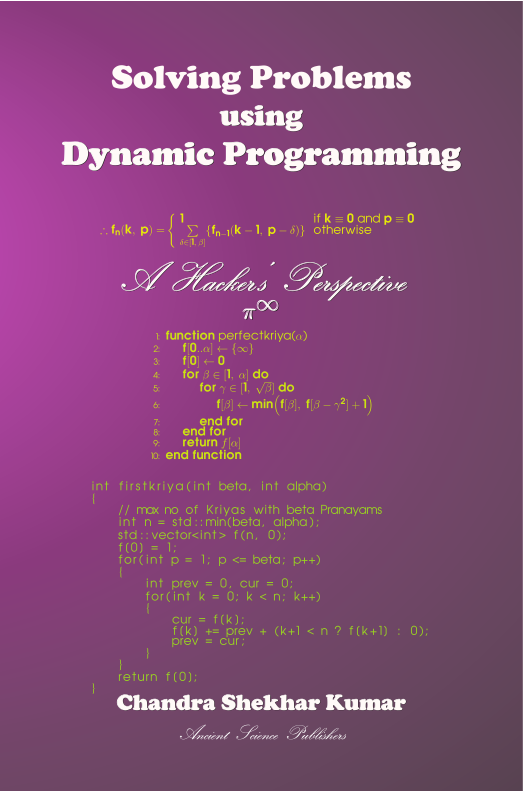
\includegraphics[width=0.5\textwidth]{solvingdpp/cover/dpp-cover}
  \end{center}
  %\caption{Front Cover}
\end{wrapfigure}
\end{warpHTML}

\hspace{5mm}A hacker's approach to a coding problem is beyond the foundational aspect of underlying genetic and computational structures, often termed as $\color{Orange}\mathbf{\pi^\infty}$.  

\begin{warpprint}
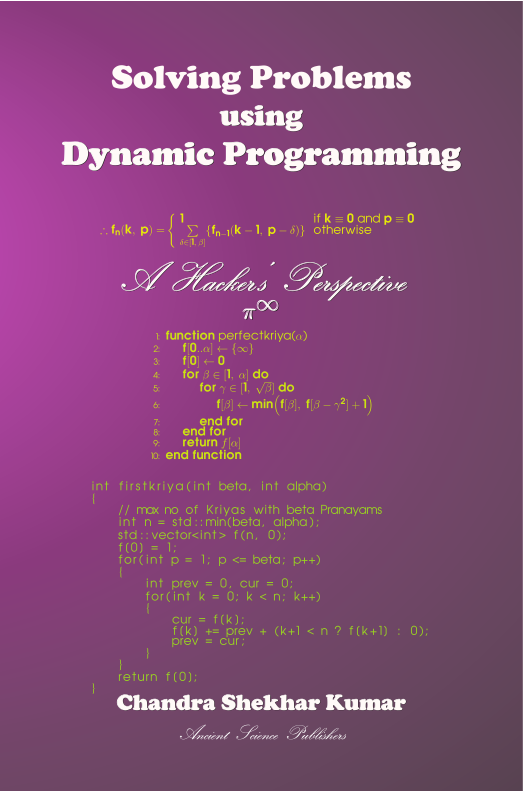
\includegraphics[width=0.5\linewidth]{solvingdpp/cover/dpp-cover}
\end{warpprint}

\hspace{5mm}A concept becomes \hlt{not difficult} because the \hlt{complexities} built into it are clarified. In a bid to reach the \hlt{core} of the problem, the concept is split-broken into fragments,  \hlt{complexities} are exposed and \hlt{delicate} points are examined. Then the concept is \hlt{recomposed} to make it integral and as a result, this reintegrated concept becomes sufficiently simple and comprehensible. 

\hspace{5mm}This helps build a hacker's insight to reveal the internal structure and internal logic of the concepts, algorithms and mathematical theorems.

\vspace{3mm}

This book provides a hacker's perspective to solving problems using dynamic programming. Written in an extremely lively form of problems and solutions (including code in modern C++ and pseudo style), this leads to extreme simplification of optimal coding with great emphasis on unconventional and integrated science of dynamic Programming. Though aimed primarily at serious programmers, it imparts the knowledge of deep internals of underlying concepts and beyond to computer scientists alike.


\vspace{0.2in}

\noindent {\calligra Ancient Science Publishers}  \hfill \emph{Chandra Shekhar Kumar}

\noindent July, 2020. \hfill 256 pages \hfill ISBN  9781722497170

\vspace{5mm}

\begin{quote}
\hspace{5mm}\hlt{Beautiful (C++) code snippets. Unique yogic exposition to coding.}
\end{quote}
\hfill {\calligra Ancient Science Hackers}


\vspace{10mm}


\underline{\textbf{\textcolor{BurntOrange}{Excerpt from the Chapter} \textcolor{Sepia}{(Optimal Loot Partition):}}}


\begin{p}
\hlt{The head of a gang of robbers embarks on distribution of the looted amount $l (> 0)$, starting with division into two parts : $x$ and $l - x$ for $0 \le x \le l$. From $x$ : they get a return of $u(x)$ such that they are left with a lesser amount $\alpha x$ : $0 < \alpha < 1$ and from $l - x$ : a return of $v(l - x)$ such that they are left with a lesser amount $\beta(l - x)$ : $0 < \beta < 1$. So the total amount left after the first step of division is $\alpha x + \beta (l - x)$ and the process continues. Devise the partition strategy to help them maximize the return obtained in a finite $n$ or infinite number of steps.}
\end{p}

\begin{s}
Let $y(x)$ denote the return after the first step:
\begin{gather*}
\therefore y(x) = u(x) + v(l - x)
\end{gather*}
Assuming $u$ and $v$ to be continuous functions, it is trivial to find the maximum of $y(x)$ over $x \in [0, l]$ using calculus (or graphical approach) :
\begin{gather*}
\dfrac{d y}{d x} = \dfrac{d}{d x} u(x) + \dfrac{d}{d x} v(l - x) = 0 \text{ (for extrema)}.
\end{gather*}
Solve for $x$ and $y(x)$ is maximum for that $x$ for which $\dfrac{d^2 y}{d x^2} < 0$.

Suppose $u(x) = x$ and $v(l - x) = -(l - x)^2 $, then 
\begin{gather*}
y = x - (l - x)^2 \\
\therefore \dfrac{d y}{d x} = 1 + 2(l - x) = 0, \\
\therefore x = l + \dfrac{1}{2}.\\
\dfrac{d^2 y}{d x^2} = -2 < 0. \\
\therefore y_{max} = l + \dfrac{1}{2} - \dfrac{1}{4} = l + \dfrac{1}{4}. 
\end{gather*}
After the first step, the initial amount $l$ is reduced to $l_1$(say):
\begin{gather*}
\therefore l_1 = \alpha x + \beta (l - x) 
\end{gather*}
In the second step, $l_1$ is partitioned into $x_1$ (say) and $(l_1 - x_1)$ for $0 \le x_1 \le l_1$. Hence, the return from the second step is $u(x_1) + v(l_1 - x_1)$. Therefore, the total return after the two steps is:
\begin{gather*}
\therefore y(x, x_1) = u(x) + v(l - x) + u(x_1) + v(l_1 - x_1).
\end{gather*}
Maximum of the function $y(x, x_1)$ over the 2-dimensional space $(x, x_1)$ yields the maximum return, such that $x \in [0, l]$ and $x_1 \in [0, l_1]$.

Similarly, the total return after $n$ steps is :
\begin{gather}
\therefore y(x, x_1, x_2, \ldots, x_{n - 1}) = u(x) + v(l - x) + \sum_{i=1}^{n - 1}\left[u(x_i) + v(l_i - x_i)\right].
\end{gather}

Here $x_i \in [0, l_i]$.

\vspace{2mm}

Using this \emph{enumerative} approach to maximize the $n$-dimen-sional return, the computation procedure soon becomes cumbersome, error-prone and exponential in nature. 

\vspace{2mm}

Any choice of $x, x_1, x_2, \ldots$ is a \emph{policy}.

The policy maximizing $y(x, x_1, x_2, \ldots)$ is an \emph{optimal policy}.

\vspace{2mm}

It can be noted that each step depends on the respective policy only. Hence at the $(i + 1)^{th}$ step, the corresponding \emph{one-dimensional} choice is made : a choice of $x_i \in [0, l]$.

\vspace{2 mm}

Hence an optimal policy leads to the corresponding maximum return.

Let $y_n (l)$ denote the maximum total return, given the initial amount $l$ and n steps.
\begin{gather*}
\therefore y_1 (l) =  \Max\limits_{x \in [0, l]} \left[u(x) + v(l - x)\right].
\end{gather*}
After the first step, $l$ becomes $\alpha x + \beta (l - x)$ :
\begin{gather*}
\therefore y_2 (l) = \Max\limits_{x \in [0, l]} \left[u(x) + v(l - x) + y_1\left(\alpha x + \beta (l - x)\right) \right].
\end{gather*}
This leads to a recurrence relation :
\begin{gather}
\therefore y_n (l) = \Max\limits_{x \in [0, l]} \left[u(x) + v(l - x) + y_{n - 1} \left(\alpha x + \beta (l - x)\right) \right] . \label{lootpartition:e1}
\end{gather}

Hence a single $n$-dimensional problem is reduced to a sequence of $n$ one-dimensional problems.

Here, the optimal return depends on the initial amount $l$ and initial decision of division into the parts $l$ and $l - x$ only.

\vspace{2 mm}

This is possible due to \hlbt{the Principle of Optimality} : 
\begin{quote}
\hlt{An optimal policy has the property that whatever the initial state and initial decision are, the remaining decisions must constitute an optimal policy with regard to the state resulting from the first decision.}
\end{quote}
Hence~\cref{lootpartition:e1} is the required optimal strategy.
%\par \vspace{-1.9\baselineskip}
%\qedhere
\end{s}




\vspace{15mm}


\underline{\textbf{\textcolor{BurntOrange}{Excerpt from the Chapter} \textcolor{Sepia}{(Constrained Subsequence):}}}


\section*{Maximum Sum}\index{Constrained Subsequence!Maximum Sum}
\begin{p} \label{maxsubarray : sum}\index{Max Sum Subarray}
Given a sequence of $n \in (-\infty, \; \infty)$ integers, determine the largest possible sum of the contiguous subsequence.
\end{p}

\begin{s}
Let $f_n(i)$ be the maximum sum of a contiguous subsequence ending at index $i$, obtained using an optimal policy and $n$ steps.

Let $s_i$ be the value of the element at index $i$, i.e. $s_i$ is used at the $n^{th}$ step. The we can use an optimal policy starting with previously accumulated maximum sum of a contiguous subsequence ending at index $i-1$.

Hence the required optimal procedure is
\begin{align*}
\therefore f_n(i) &= \Max\limits_{i \in [0, \; n-1]} \left[f_{n-1}(i-1) + s_i\right]
\end{align*}

At each step (with addition of $s_i$), there are 2 options :
\begin{enumerate}
    \item leverage the previous accumulated maximum sum if \\$f_{n-1}(i-1) + s_i > 0$, because it is better to continue with a positive running sum or
    \item start afresh with a new range (with the starting sum as 0) if $f_{n-1}(i-1) + s_i < 0$, because it is better to start with 0 than continuing with a negative running sum. 
\end{enumerate} 

Also note that:
\begin{itemize}
    \item If all the elements are negative, then there is no such subsequence, i.e. the required sum is 0.
    \item If all the elements are positive, then the entire sequence is the required subsequence, i.e. the required sum is the sum of all the elements of the sequence.  
    \item The required subsequence (if any) starts at and ends with a positive value.
\end{itemize}



\begin{figure}
\begin{center}
\fbox{\hlbt{Maximum sum contiguous subsequence : compute sum}}
\end{center}
\begin{algorithmic}[1]
\Function{maxseq}{$s[0..n-1]$}
    \State $currentsum \gets 0$
    \State $maxsum \gets 0$
    \For{$x \in s[0 .. n-1]$}
        \State $currentsum \gets$ \textbf{max}$(currentsum + x, 0)$
        \State $maxsum \gets$ \textbf{max}$(maxsum, currentsum)$ 
    \EndFor
    \State \textbf{return} $maxsum$
\EndFunction
\end{algorithmic}
\end{figure}

Time complexity is $\bigO(n)$. Space complexity is $\bigO(1)$.

\begin{lstlisting}
int maxseq(std::vector<int> & s)
{
    int current_sum = 0;
    int max_sum = 0;

    for(int x : s)
    {
        current_sum = std::max(current_sum + x, 0);
        max_sum = std::max(max_sum, current_sum);
    }
    return max_sum;
}
\end{lstlisting}
\par \vspace{-1.2\baselineskip}
\qedhere
\end{s}


\section*{Circular Sequence}\index{Constrained Subsequence!Circular Sequence}

\begin{p}\label{maxcircular:p1}
Given a circular sequence $s$ of $n \in (-\infty, \infty)$ integers, find the maximum possible sum of a non-empty contiguous subsequence of $s$.
\end{p}

\begin{s}
The end of a circular sequence wraps around the start of the sequence itself, i.e.
\begin{gather*}
\because i \equiv (i + n) \; \mathbf{mod} \; n \quad \forall i \in [0, n) \\
\therefore s_i \equiv s_{(i+n) \; \mathbf{mod} \; n} \quad \forall i \in [0, n).
\end{gather*}

\begin{center}
\begin{tikzpicture} %[nodes in empty cells,
      %nodes={minimum width=0.5cm, minimum height=0.5cm},
      %row sep=-\pgflinewidth, column sep=-\pgflinewidth]
      %border/.style={draw}
    
      \matrix(vector)[matrix of nodes, row sep=0.2cm, column sep=-\pgflinewidth, nodes={draw, minimum width=11mm, minimum height=5mm}] (m)
      {
          $s_{0}$ & $s_{1}$ & $\ldots$ & $s_{i}$ & $\ldots$ & $s_{n-1}$\\
          $s_{n}$ & $s_{n+1}$ & $\ldots$ & $s_{n+i}$ & $\ldots$ & $s_{2n-1}$\\
      };
      \foreach \i in {1,...,6}
      {
          \draw[->] (m-2-\i) -- (m-1-\i);
       }
\end{tikzpicture}
\end{center}

For a maximum contiguous subsequence $\mleft[s_i \cdots s_j\mright]$, the solution of~\cref{maxsubarray : sum} can be used.

\begin{center}
\begin{tikzpicture}[
    MyStyle/.style={draw, minimum width=2em, minimum height=2em, 
                outer sep=0pt},
  ]

\matrix (A) [matrix of math nodes, nodes={MyStyle, anchor=center}, column sep=-\pgflinewidth]
{s_0 & \cdots & s_i & s_{i+1} & \cdots & s_{j-1} & s_j & \cdots & s_{n-1}\\};

\draw[decorate,decoration={brace, amplitude=10pt, raise=2pt, mirror}]
  (A-1-3.south west) to node[black,midway,below= 10pt] {max subsequence} (A-1-7.south east);%
\end{tikzpicture}
\end{center}

For a maximum contiguous subsequence $\mleft[s_j \cdots s_{n-1}, s_0 \cdots s_i\mright]$, the left-over part $\mleft[s_{i+1} \cdots s_{j-1}\mright]$ forms a minimum contiguous subsequence.\index{Min Sum Circular Subarray}

\begin{center}
\begin{tikzpicture}[
    MyStyle/.style={draw, minimum width=2em, minimum height=2em, 
                outer sep=0pt},
  ]

\matrix (A) [matrix of math nodes, nodes={MyStyle, anchor=center}, column sep=-\pgflinewidth]
{s_0 & \cdots & s_i & s_{i+1} & \cdots & s_{j-1} & s_j & \cdots & s_{n-1}\\};

\draw[decorate,decoration={brace, amplitude=10pt, raise=2pt, mirror}]
  (A-1-1.south west) to node[black,midway,below= 10pt] {\scriptsize max subseq part 2} (A-1-3.south east);%
\draw[decorate,decoration={brace, amplitude=10pt, raise=2pt, mirror}]
  (A-1-7.south west) to node[black,midway,below= 10pt] {\scriptsize max subseq part 1} (A-1-9.south east);%
  
  \draw[decorate,decoration={brace, amplitude=10pt, raise=2pt, mirror}]
  (A-1-6.north east) to node[black,midway,above= 10pt] {\scriptsize min subsequence} (A-1-4.north west);%
\end{tikzpicture}
\end{center}

Summation of the contiguous subsequence \\$\mleft[s_j \cdots s_{n-1}, s_0 \cdots s_i\mright]$ is
\begin{align*}
&= s_j + \cdots + s_{n-1} + s_0 + \cdots + s_i \\
&= s_0 + \cdots + s_{n-1} - \mleft[s_{i+1} + \cdots + s_{j-1} \mright]
\end{align*}
This is maximum when $\mleft[s_{i+1} + \cdots + s_{j-1} \mright]$ is minimum.
\begin{gather*}
\therefore \Max \mleft[s_j + \cdots + s_{n-1} + s_0 + \cdots + s_i\mright] = \sum\limits_{k=0}^{k=n-1} s_k - \Min \sum\limits_{k=i+1}^{k=j-1} s_k \\
\therefore \text{Maximum sum subsequence } = \text{ Total sum of the sequence } \\
\quad\quad\quad\qq{}\qq{}\qq{} \qq{}\qq{}\qq{} - \text{ Minimum sum subsequence}
\end{gather*}


\begin{figure}
\begin{center}
\fbox{\hlbt{Maximum sum circular subsequence}}
\end{center}
\begin{algorithmic}[1]
\Function{maxcircularseq}{$s[0..n-1]$}
    \State $currentmax \gets 0$
    \State $maxsum \gets -\infty$
    \State $currentmin \gets 0$
    \State $minsum \gets \infty$
    \State $totalsum \gets 0$
    \Statex
    \For{$x \in s[0 .. n-1]$}
        \State $currentmax \gets$ \textbf{max}$(currentmax + x, x)$
        \State $maxsum \gets$ \textbf{max}$(maxsum, currentmax)$ 
        \Statex
        \State $currentmin \gets$ \textbf{min}$(currentmin + x, x)$
        \State $minsum \gets$ \textbf{min}$(minsum, currentmin)$ 
        \Statex
        \State $totalsum \gets totalsum + x$
    \EndFor
    \Statex
    \If{$totalsum == minsum$} \Comment{All elements are -ve}
        \State \textbf{return} $maxsum$ \Comment{Value of the least -ve element}
    \Else
        \State \textbf{return} \textbf{max}$(maxsum, \; totalsum - minsum)$
    \EndIf
\EndFunction
\end{algorithmic}
\end{figure}

Time complexity is $\bigO(n)$. Space complexity is $\bigO(1)$.

\begin{lstlisting}
int maxsum_circular(std::vector<int> & s)
{
    int current_max = 0, max_sum = std::numeric_limits<int>::min();
    int current_min = 0, min_sum = std::numeric_limits<int>::max();
    int total_sum = 0;

    for(int x : s)
    {
        current_max = std::max(current_max + x, x);
        max_sum = std::max(max_sum, current_max);

        current_min = std::min(current_min + x, x);
        min_sum = std::min(min_sum, current_min);

        total_sum += x;
    }
    // when all elements are -ve => total_sum == min_sum, 
    // i.e. total_sum - min_sum becomes 0 => empty subsequence
    // but max_sum still holds the value of the least -ve element,
    // hence return this singleton than an empty one
    return total_sum == min_sum ? max_sum : std::max(max_sum, total_sum - min_sum);
}
\end{lstlisting}

\begin{comment}
\begin{center}
\scalebox{0.9}{
\begin{tabular}{ccc} \hline
\textbf{Circular Sequence} & \textbf{Max Sum Subsequence} & \textbf{Max Sum} \\ \hline
1,-2,3,-2 & 3 & 3\\ \hline
5,3,-5 & 5,5 & 10 \\ \hline
3,-1,2,-1 & 3,-1,2 and 2, -1, 3 & 4 \\ \hline
3,-2,2,-3 & 3 and 3,-2,2 & 3 \\ \hline
-2,-3,-1 & -1 & -1 \\ \hline
8,-1,3,4 & 3,4,8 & 15 \\ \hline
5,-3,5,5,-3 & 5,-3,5,5 and 5,5,-3,5 & 12 \\ \hline
\end{tabular}}
\end{center}
\par\vspace{-0.5\baselineskip}
\qedhere
\end{comment}
\end{s}


\section*{Brief Table of Contents}

\begin{enumerate}[noitemsep]
\item Genesis
    \begin{enumerate}
        \item Optimal Loot Partition
         \begin{enumerate}
             \item Deterministic
             \item Stochastic
         \end{enumerate}
        \item Exam Prep
        \item Optimal Coin Tossing
        \item Proving Optimality Principle
    \end{enumerate}
\item Computation
    \begin{enumerate}
        \item Ascension to Heaven
        \item Fibonacci Line Search
        \item Coin Change
        \item Constrained Subsequence
            \begin{enumerate}
                \item Maximum Sum 
                \item Minimum Sum 
                \item Circular Sequence 
                \item Maximum Product 
           \end{enumerate}
           \item Stock Trading 
           \item Binary Tree Mall Loot 
           \item Binary Search Tree Generation
           \item Quantify Yogic Effect
           \item Path to Heaven
            \begin{enumerate}
              \item Stairway
              \item Kriya Grid
           \end{enumerate}
           \item Kriya Sequence
           \item Kriya Catalysis
    \end{enumerate}
\end{enumerate}


\section*{List of Algorithms/Programs}
\begin{enumerate}[noitemsep]
    \item Minimum Coin Change : Iterative (Bottom-up) Approach 
    \item Minimum Coin Change : Recursive (Top-down) Approach 
    \item Minimum Coin Change : Optimal set of coins 
    \item Coin Change : No of Ways 
    \item Maximum sum contiguous subsequence : compute sum
    \item Maximum sum contiguous subsequence : compute indices 
    \item Maximum sum non-contiguous subsequence : compute sum 
    \item Maximum sum non-contiguous subsequence : compute sum : space optimized
    \item Minimum sum contiguous subsequence .
    \item Min sum contiguous subsequence : Find max of -ve 
    \item Minimum sum contiguous subsequence : compute indices 
    \item Maximum sum circular subsequence 
    \item Minimum sum circular subsequence 
    \item Maximum product contiguous subsequence : compute product 
    \item Maximum product contiguous subsequence : compute product : modified 
    \item Stock Trading : Maximum Profit : One Transaction 
    \item Maximize Profit : Maximum sum contiguous subsequence
    \item Maximize Profit : Buy and Sell Days 
    \item Stock Trading : Maximum Profit : Two Transactions 
    \item Stock Trading : Maximum Profit : m(< n) Transactions 
    \item Stock Trading : Maximum Profit : m(> n) or Unlimited Transactions 
    \item Stock Trading : Maximum Profit : m(> n) or Unlimited Transactions : Alternative
    \item Count Unique BSTs 
    \item Generate Unique BSTs
    \item Quantify Yogic Effect : Drink Air Therapy
    \item Quantify Yogic Effect : Khechari Kriya 
    \item Quantify Yogic Effect : Mool Kriya 
    \item Quantify Yogic Effect : Tandav Kriya 
    \item Quantify Yogic Effect : Minimax Kriya Selection .
    \item Quantify Yogic Effect : Minimax Kriya Selection : Optimized Computation 
    \item Quantify Yogic Effect : Trikaldarshi 
    \item Quantify Yogic Effect : Trikaldarshi : Print Kriya Triangles 
    \item Staircase to Heaven : Count Distinct Ways 
    \item Staircase to Heaven : Count Distinct Ways with step-list 
    \item Staircase to Heaven : Optimal Pranayams 
    \item Distinct Kriya Grid Paths to Heaven 
    \item Distinct Kriya Grid Paths to Heaven : Space Optimization 
    \item Distinct Kriya Grid Paths to Heaven : With Prohibition 
    \item Distinct Kriya Grid Paths to Heaven : With Prohibition : Space Optimization
    \item Distinct Kriya Grid Paths to Heaven : With Prohibition : Space Optimization : Alternative
    \item Kriya Grid Paths to Heaven : Optimal Pranayams
    \item Constrained Kriya Grid Paths to Heaven : Optimal Pranayams
    \item Constrained Kriya Grid Paths to Heaven : Optimal Pranayams : Diff Cols
    \item Constrained Kriya Grid Paths to Heaven : Optimal Pranayams : Diff Cols : Optimized 
    \item Optimal Pranayams to reach Heaven 
    \item Count ways : First Kriya 
    \item Count ways : First Kriya : Space Optimization 
    \item Out of Kriya Grid : Count ways 
    \item Out of Kriya Grid : Count ways : Space Optimization 
    \item Triangular Kriya Grid : Optimal Pranayams 
    \item Triangular Kriya Grid : Optimal Pranayams : Alternative
    \item Maximal Square Kriya Grid 
    \item Max Zerones Kriya Sequences 
    \item Perfect Kriya
    \item Generate Kriya 
    \item Vanish Kriya 
    \item Split Kriya
    \item Threshold Kriya 
    \item Threshold Kriya : Space Optimization
    \item Rejuvenate Kriya
    \item Rejuvenate Kriya : Space Optimization
    \item $\beta$-Dimensional Kriya
    \item $\beta$-Dimensional Kriya : Space Optimization 
    \item Kriya Moves
    \item Marking Kriya
    \item Marking Kriya : Space Optimization 
    \item Kriya Selection 
    \item Kriya Sets : Possible Moves 
    \item Kriya Sets : Space Optimization 
    \item Count Distinct Pranayams Sets
    \item Partition Kriya : Iso-Pranayams Sets 
    \item Partition Kriya : Iso-Pranayams Sets : Space Optimization
    \item Kriya Probability 
    \item  Combine Kriya 
    \item  Sort Kriya : Optimal Interchanges
    \item  Sort Kriya : Space Optimization 
    \item  Longest Increasing Subsequence (LIS) of Kriyas 
    \item  Permute Kriyas 
    \item  Length of LCS Kriya 
    \item  LCS Kriya
    \item  Compute and Print LCS Kriya
    \item  Compute and Print LCS Kriya : Alternative 
    \item  Compute All The LCS Kriya
    \item  Length of LCS Kriya : Space Optimization
    \item  Length of SCS Kriya 
    \item  Reconstruction of SCS Kriya from Optimal Solution 
    \item  Print SCS : Recursive Approach
    \item  Compute All The SCS Kriya 
    \item  Computation SCS from LCS Kriya
    \item  SCS Kriya : Alternative Solution from LCS 
    \item  Counting Palindromic Kriya Contiguous Subsequence 
    \item  Longest Palindromic Kriya Contiguous Sub sequences
    \item  Maximum Length of Palindromic Kriya Subsequence 
    \item  Max Length of Palindromic Kriya Subsequence : Alternative
    \item  Maximum Length of Palindromic Kriya Subsequence : Space Optimization 
    \item  Max Length of Palindromic Kriya Subsequence : Space Optimization : Alternative 
    \item  Count of Distinct Kriya Subsequences
    \item  Count of Distinct Kriya Subsequences : Space Optimization 
    \item  Transform Kriya 
    \item  Print Transformation Path 
    \item  Transform Kriya : Space Optimization
    \item Print Operations
    \item Reconstruct Operations
    \item Transform Kriya and Reconstruct Operations 
    \item Print Operations
    \item Reconstruct Operations 
    \item Transform Kriya and Reconstruct Operations 
    \item Transform Kriya : Unrestricted Operations 
    \item Edit Distance : Print Operations with Copy and Finish 
    \item Edit Distance : Print Custom Operations with Reconstruct Operations 
    \item Edit Distance : Transform Kriya and Reconstruct Custom Operations 
    \item Reconstruct and Print Aligned Kriya Sequences 
    \item Generate Aligned Kriya Sequences 
    \item Generate \& Reconstruct Aligned Kriya Sequences
    \item Identical Kriya Sequences
    \item Identical Kriya Sequences with Reconstruction 
    \item Identical Kriya Sequences : Reconstruction (Recursive) 
    \item Generate Identical Kriya Sequences with Reconstruction (Recursive) 
    \item Generate Identical Kriya Sequences : Optimal Space
    \item Optimal Removed Kriyas 
    \item Kriya Sequence Generation : Count Ways : Constraints of Favourable Comparisons 
    \item Preferred Kriya Practice : Count Ways 
    \item Preferred Kriya Practice : Count Ways : Space Optimization
    \item Binary Split Kriyas : Count Ways 
    \item Organize Kriyas : Ways of Non-adjacent ones 
    \item Select Kriyas Alternately : Optimal Difference 
    \item Decode Kriya Sequence from Digits Sequence 
    \item Sorted Kriya Sequence : Transduction Quotient 
    \item Cross Kriya Potential
    \item Maximum Sum : Linear and Circular Kriya Sequence
\end{enumerate}










%\begin{warpHTML}
%\href{solvingdpp/dpp.html}{solvingdpp/dpp.html}
%\end{warpHTML}
%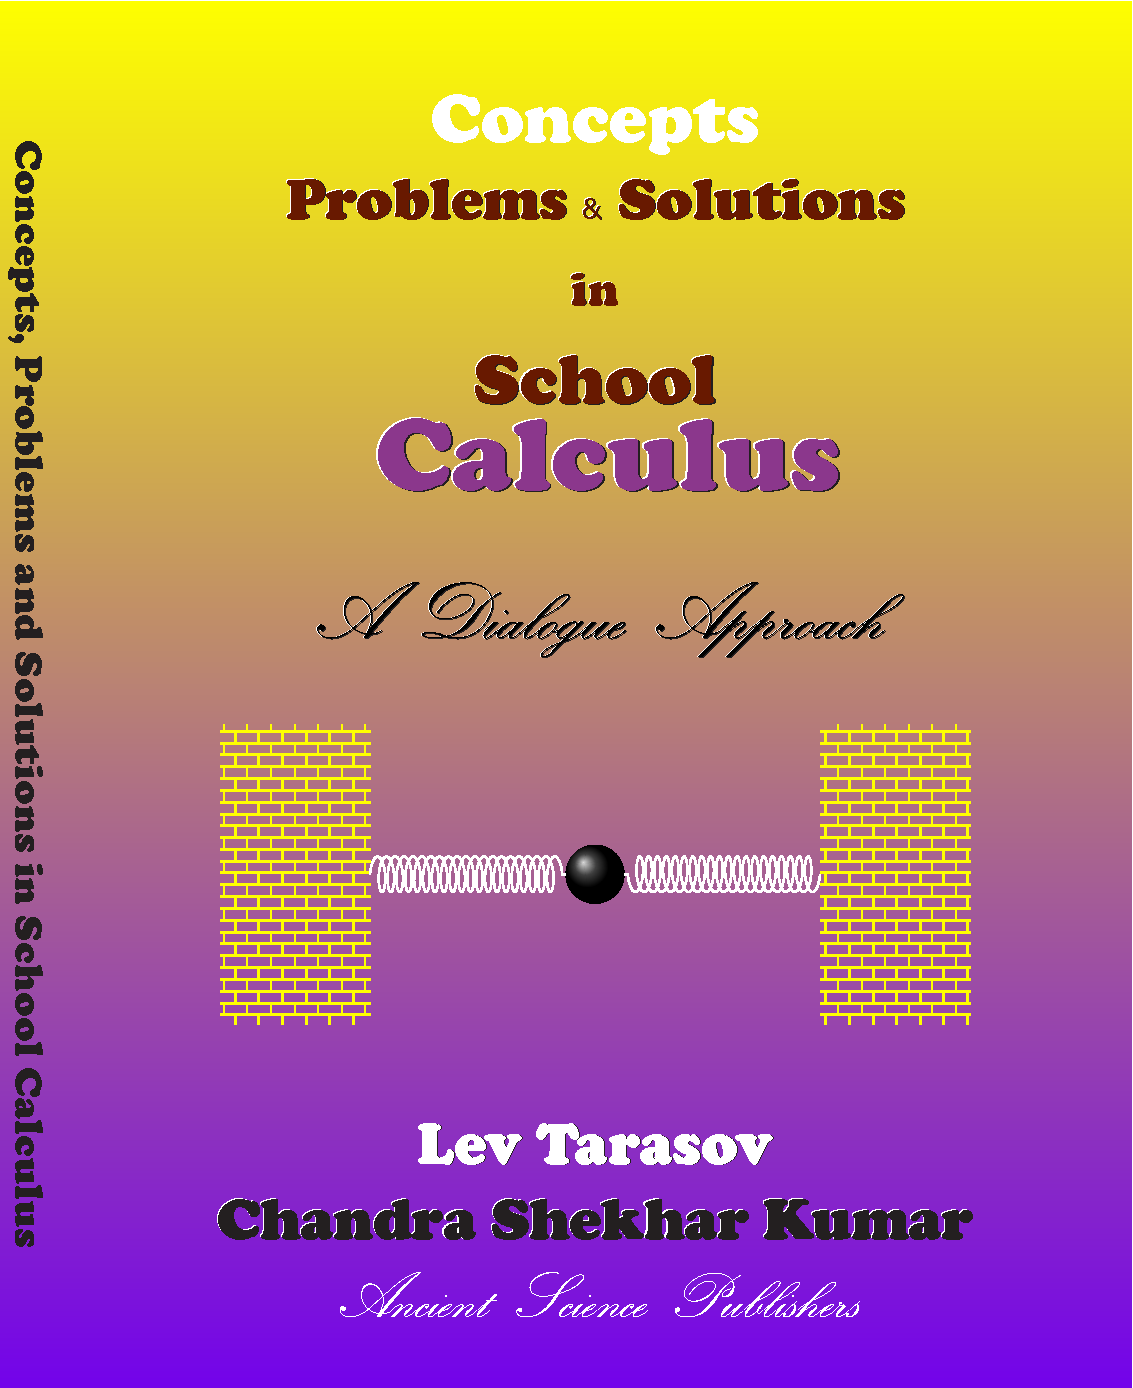
\includegraphics{solvingdpp//cover}

\chapter{Hacking TensorFlow Internals : An Insider’s Commentary on A Learning System}

\chapter{Advanced C++ FAQs Vol 1 \& 2}

\chapter{C++14 FAQs}

\chapter{The Boost C++ Libraries: Generic Programming}

\chapter{Generic Algorithms and Data Structures using C++11}

\chapter{C++11 Standard Library: Usage and Implementation}

\chapter{Foundation of Algorithms in C++11}

\chapter{C++11 Algorithms : Using and Extending C++11, Boost and Beyond}

\chapter{Cracking Programming Interviews : 500 Questions with Solutions}

\chapter{Top 20 Coding Interview Problems Asked in Google with Solutions}

\chapter{Top 10 Coding Interview Problems Asked in Google with Solutions}



\part{Physics}
PHY

\part{Mathematics}
MATH

\end{document}